\documentclass[11pt,letterpaper]{article}
\usepackage[lmargin=1in,rmargin=1in,tmargin=1in,bmargin=1in]{geometry}
\usepackage{../style/homework}
\usepackage{../style/commands}
\setbool{quotetype}{true} % True: Side; False: Under
\setbool{hideans}{true} % Student: True; Instructor: False

% -------------------
% Content
% -------------------
\begin{document}

\homework{7: Due 10/02}{This is the worst kind of discrimination --- the kind against me!}{Bender Bending Rodr\'iguez, Futurama}

% Problem 1
\problem{10} Consider the function given by $W(t)= 568.1 - 13.4t$. 
	\begin{enumerate}[(a)]
	\item Is $W(t)$ a linear function? Explain.
	\item Find the slope of $W(t)$.
	\item Find the $y$-intercept of $W(t)$.
	\item Find the $x$-intercept of $W(t)$. 
	\item Find a value of $t$ for which $W(t)= 100$. 
	\end{enumerate}



\newpage



% Problem 2
\problem{10} Consider the relation plotted below.
	\[
	\fbox{
	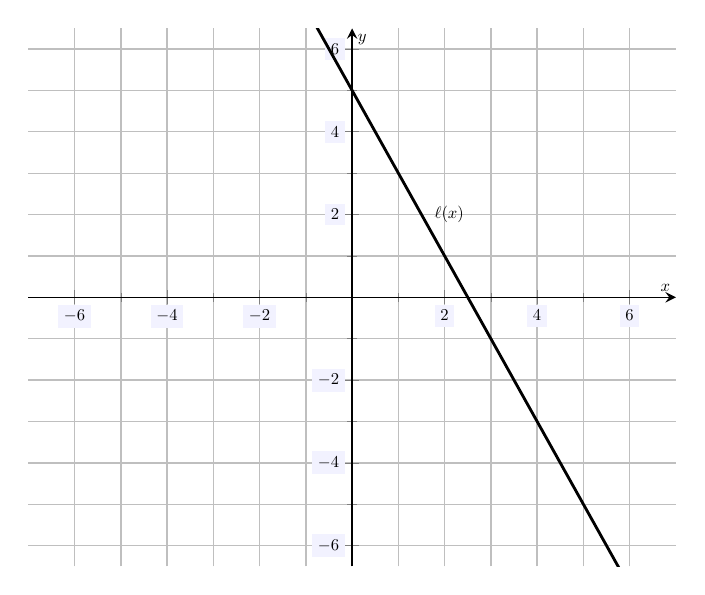
\begin{tikzpicture}[scale=1.2,every node/.style={scale=0.5}]
	\begin{axis}[
	grid=both,
	axis lines=middle,
	ticklabel style={fill=blue!5!white},
	xmin= -7, xmax=7,
	ymin= -6.5, ymax=6.5,
	xtick={-6,-4,-2,0,2,4,6},
	ytick={-6,-4,-2,0,2,4,6},
	minor tick = {-5,-3,...,5},
	xlabel=\(x\),ylabel=\(y\),
	]
	\addplot[domain=-7:7, samples=100,line width=0.03cm] (x,5 - 2*x);
	\node at (2.1,2) {$\ell(x)$};
	\end{axis}
	\end{tikzpicture}
	}
	\]

\begin{enumerate}[(a)]
\item Is $\ell(x)$ a linear function? Explain.
\item Find the equation for $\ell(x)$. 
\item Find the $x$ and $y$-intercepts for $\ell(x)$. 
\item Find a value of $x$ for which $\ell(x)= -3$. 
\end{enumerate}



\newpage



% Problem 3
\problem{10} Consider the linear function that goes through the points $(-4, 5)$ and $(6, 0)$.
	\begin{enumerate}[(a)]
	\item Find the slope of this linear function.
	\item Find the equation of this linear function.
	\end{enumerate}



\newpage



% Problem 4
\problem{10} A certain product requires \$800 of upfront costs to produce---the \textit{fixed costs}. After this investment, it costs \$8.50 produce every item. 
	\begin{enumerate}[(a)]
	\item Explain why the cost to produce $q$ items, $C(q)$, is a linear function.
	\item Find the equation for $C(q)$.
	\item What does the $y$-intercept for $C(q)$ represent?
	\item How much does it cost to produce 10,000~items?
	\item What is the maximum number of items you could produce with \$6,000?
	\end{enumerate}


\end{document}